\chapter{Нелінійні Алгоритми Машинного Навчання.}

До цього моменту ми ілюстрували лінійну регресію як «проведення лінії через дані», 
але насправді це було функцією наших вхідних характеристик.

Хоча це може здаватися обмеженим, алгоритми лінійної регресії є досить потужними, коли застосовуються 
до нелінійних характеристик вхідних даних.

Розглянемо, для прикладу, дані про ріст ВВП Китаю за останні 60 років, і спробуємо побудувати модель, що дає найкраще передбачення.

\begin{lstlisting}
import matplotlib.pyplot as plt
import pandas as pd

def build_plot(file_path, x, y):
    data = pd.read_csv(file_path)
    plt.scatter(data[x], data[y], c='blue', marker='x')
    plt.xlabel(x)
    plt.ylabel(y)
    return plt
    # plt.show()

build_plot('../resources/china_gdp.csv', 'Year', 'Value').show()
\end{lstlisting}

Результат:

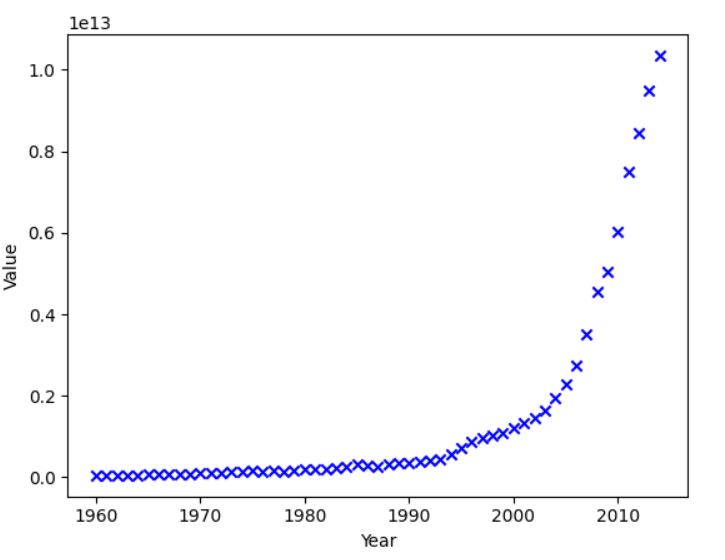
\includegraphics[scale=0.75]{img/203-1}

Якщо спробувати провести лінію через цей графік, отримаємо наступне:

\begin{lstlisting}
plt = build_plot('../resources/china_gdp.csv', 'Year', 'Value')
data = pd.read_csv('../resources/china_gdp.csv')
x, y = data['Year'], data['Value']
x_reshaped, y_reshaped = x.values.reshape(-1, 1), y.values.reshape(-1, 1)

from sklearn.linear_model import LinearRegression
import numpy as np

model = LinearRegression(fit_intercept=True)
model.fit(x_reshaped, y_reshaped)
Xnew = np.array([[2025], [2030]])
print(model.predict(Xnew))

theta = [ model.coef_[0], model.intercept_ ]
print(theta)

X_line = np.linspace(x_reshaped.min(), x_reshaped.max(), 100).reshape(-1, 1)
y_line = model.predict(X_line)

plt.plot(X_line, y_line)
\end{lstlisting}

Результат:

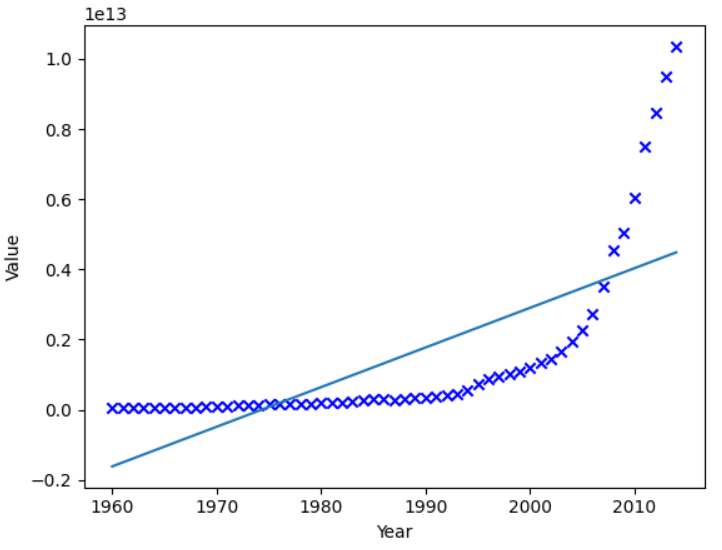
\includegraphics[scale=0.75]{img/203-2}

Очевидно, що лінійна модель не найкращим чином наближає ці дані.

Нелінійна модель машинного навчання — це модель, яка здатна описувати складні, нелінійні залежності між вхідними ознаками та цільовою змінною. На відміну від лінійних моделей, вона не обмежується прямою або площиною як межею прогнозування, а може будувати криволінійні поверхні, що точніше відображають закономірності реальних даних.




\section{Поліноміальна Регресія.}

Поліноміальна регресія — це різновид лінійної регресії, в якому взаємозв’язок між 
$x$ та $y$ моделюється у вигляді полінома $n$-го ступеня:

$$y = \beta_{0} + \beta_{1} x + \beta_{2} x^{2} + ... + \beta_{n} x^{n} + \epsilon$$

Це дозволяє моделювати нелінійні залежності шляхом додавання поліноміальних членів ознак.

Щоб використати поліноміальну регресію, достатньо імпортувати відповідний модуль:

\begin{lstlisting}
from sklearn.preprocessing import PolynomialFeatures
\end{lstlisting}

Та трансформувати вхідні ознаки в поліноміальні:

\begin{lstlisting}
poly = PolynomialFeatures(degree=5)
X_poly = poly.fit_transform(x_reshaped)
\end{lstlisting}

Разом код виглядає наступним чином:

\begin{lstlisting}
import numpy as np
import matplotlib.pyplot as plt
from sklearn.linear_model import LinearRegression
from sklearn.preprocessing import PolynomialFeatures

plt = build_plot('../resources/china_gdp.csv', 'Year', 'Value')
data = pd.read_csv('../resources/china_gdp.csv')
x, y = data['Year'], data['Value']
x_reshaped, y_reshaped = x.values.reshape(-1, 1), y.values.reshape(-1, 1)

poly = PolynomialFeatures(degree=5)
X_poly = poly.fit_transform(x_reshaped)

# model fit:
model = LinearRegression()
model.fit(X_poly, y_reshaped)

# forecast and visualization:
X_plot = np.linspace(min(x_reshaped), max(x_reshaped), 100).reshape(-1, 1)
y_pred = model.predict(poly.transform(X_plot))

plt.scatter(x, y, color='blue', label='Data points')
plt.plot(X_plot, y_pred, color='red', label='Polynomial fit')
plt.xlabel("X")
plt.ylabel("y")
plt.title("Polynomial Regression (degree=5)")
plt.legend()
plt.show()

# coefficients
print("Intercept:", model.intercept_)
print("Coefficients:", model.coef_)
\end{lstlisting}

Результат:

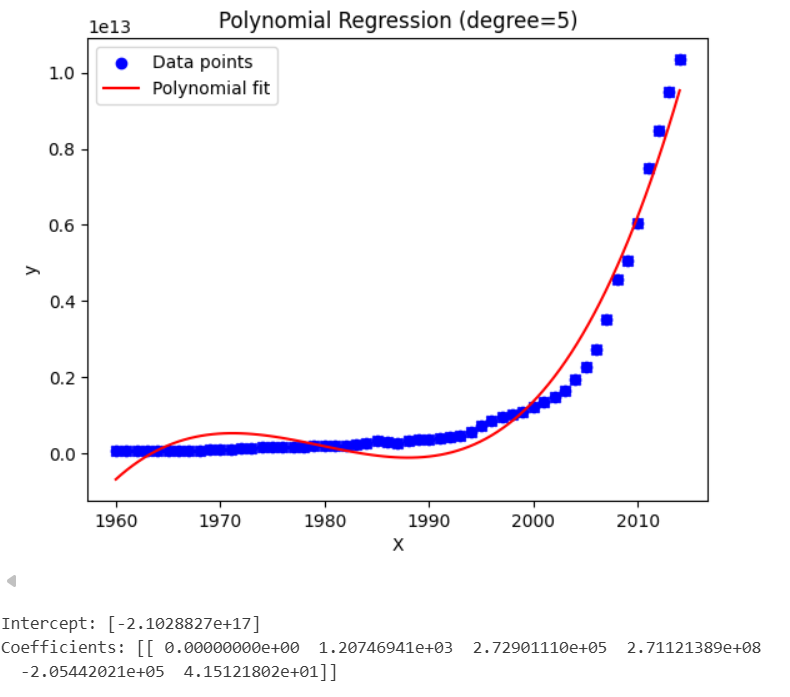
\includegraphics[scale=0.75]{img/203-3}



\subsection{Узагальнення та перенавчання.}

Проблема з канонічною задачею машинного навчання полягає в тому, що нас насправді не цікавить мінімізація цієї цілі на заданому наборі даних.

Нас насправді цікавить, наскільки добре наша функція узагальниться на нових прикладах, які ми не використовували для навчання системи (але які взяті з «того самого розподілу», що й приклади, які ми використовували для навчання)

Поліноми вищого ступеня демонстрували перенавчання: вони фактично мають дуже низькі втрати на даних навчання, але створюють функції, які, як ми очікуємо, не будуть добре узагальнюватися.

У міру ускладнення моделі втрати навчання завжди зменшуються; втрати узагальнення зменшуються до певної точки, а потім починають збільшуватися

Хоча важко кількісно оцінити справжню помилку узагальнення (тобто помилку цих 
алгоритмів щодо повного розподілу можливих прикладів), ми можемо 
наблизити її за допомогою \textit{перехресної валідації}.

Основна ідея полягає в тому, щоб розділити набір даних на навчальний набір і набір для перевірки. Навчіть алгоритм на навчальному наборі і оцініть на наборі для перевірки.

Ми називаємо змінні $\theta$ параметрами алгоритму машинного навчання.
Але є й інші величини, які також впливають на класифікатор: ступінь полінома, 
кількість регуляризації тощо; їх сукупно називають 
гіперпараметрами алгоритму.

Основна ідея перехресного валідації: використовувати навчальний набір для визначення параметрів, використовувати 
резервний набір для визначення гіперпараметрів.


\subsection{k-кратна перехресна валідація.}

k-кратна перехресна валідація (k-folds validation) - це більш складна (але насправді дещо більш поширена) версія перехресної валідації.
Розділіть набір даних на $k$ роз'єднаних підмножин (складок); навчіть на $k-1$ і оцініть на 
залишковій складці; повторіть $k$ разів, утримуючи кожну складку один раз. Повідомте середню похибку для всіх утриманих складок.

\textbf{Варіанти.}

\begin{itemize}
\item Перехресна валідація «залиш один»: обмеження k-кратної перехресної валідації, де кожна 
складка є лише одним прикладом (тож ми навчаємося на всіх інших прикладах, тестуючи 
цей один приклад)

Дещо дивно, але для найменших квадратів це можна обчислити ефективніше, ніж k-кратну 
перехресну валідацію, з такою ж складністю вирішення для оптимального $\theta$ за допомогою матричного рівняння.

\item Стратифікована перехресна валідація: збереження приблизно рівного відсотка 
позитивних/негативних прикладів (або будь-якої іншої ознаки) у кожному згині.
\end{itemize}

\ding{43} Попередження: k-кратна перехресна валідація не завжди є кращою (наприклад, у прогнозуванні часових рядів 
бажано, щоб набір утриманих даних був повністю сформований після набору навчання)



\section{Поліноміальна класифікація.}

Наведемо приклад поліномільної класифікації на тому ж датасеті пухлин молочної залози.

Завантажуємо датасет (лише дві ознаки для класифікації: середній радіус, середній периметр)

\begin{lstlisting}
data = load_breast_cancer()
X = data.data[:, [3, 25]]
y = data.target
\end{lstlisting}

Розбиття на тренувальні та тестові дані:

\begin{lstlisting}
X_train, X_test, y_train, y_test = train_test_split(X, y, test_size=0.3, random_state=10)
\end{lstlisting}

Скейлимо дані:

\begin{lstlisting}
scaler = StandardScaler()
X_train_scaled = scaler.fit_transform(X_train)
X_test_scaled = scaler.transform(X_test)
\end{lstlisting}

Додаємо поліноміальні ознаки (нелінійна трансформація):

\begin{lstlisting}
poly = PolynomialFeatures(degree=10)
X_train_poly = poly.fit_transform(X_train_scaled)
X_test_poly = poly.transform(X_test_scaled)
\end{lstlisting}

Тренуємо логістичну регресію на поліноміальних ознаках:

\begin{lstlisting}
clf = LogisticRegression(max_iter=10000)
clf.fit(X_train_poly, y_train)
\end{lstlisting}

Евалююємо:

\begin{lstlisting}
y_pred = clf.predict(X_test_poly)
print("Accuracy:", accuracy_score(y_test, y_pred))
\end{lstlisting}

Візуалізація (Межа між класами):

\begin{lstlisting}
x_min, x_max = X_train_scaled[:, 0].min() - 1, X_train_scaled[:, 0].max() + 1
y_min, y_max = X_train_scaled[:, 1].min() - 1, X_train_scaled[:, 1].max() + 1
xx, yy = np.meshgrid(np.linspace(x_min, x_max, 200),
                     np.linspace(y_min, y_max, 200))

Z = clf.predict(poly.transform(np.c_[xx.ravel(), yy.ravel()]))
Z = Z.reshape(xx.shape)

plt.contourf(xx, yy, Z, alpha=0.2, cmap='coolwarm')
plt.scatter(X_test_scaled[:, 0], X_test_scaled[:, 1], c=y_test, cmap='coolwarm', edgecolors='k')
plt.xlabel('mean radius (scaled)')
plt.ylabel('mean perimeter (scaled)')
plt.title('Non-linear Classification with Polynomial Logistic Regression')
plt.show()
\end{lstlisting}

Матриця похибок (confusion matrix):

\begin{lstlisting}
ConfusionMatrixDisplay.from_predictions(y_test, y_pred, cmap='Blues')
plt.title("Confusion Matrix")
plt.show()
\end{lstlisting}

Все разом:

\begin{lstlisting}
import numpy as np
import matplotlib.pyplot as plt
from sklearn.datasets import load_breast_cancer
from sklearn.preprocessing import PolynomialFeatures, StandardScaler
from sklearn.linear_model import LogisticRegression
from sklearn.model_selection import train_test_split
from sklearn.metrics import ConfusionMatrixDisplay, accuracy_score

data = load_breast_cancer()
X = data.data[:, [3, 25]] 
y = data.target

X_train, X_test, y_train, y_test = train_test_split(X, y, test_size=0.3, random_state=42)

scaler = StandardScaler()
X_train_scaled = scaler.fit_transform(X_train)
X_test_scaled = scaler.transform(X_test)

poly = PolynomialFeatures(degree=10)
X_train_poly = poly.fit_transform(X_train_scaled)
X_test_poly = poly.transform(X_test_scaled)

clf = LogisticRegression(max_iter=10000)
clf.fit(X_train_poly, y_train)

y_pred = clf.predict(X_test_poly)
print("Accuracy:", accuracy_score(y_test, y_pred))

x_min, x_max = X_train_scaled[:, 0].min() - 1, X_train_scaled[:, 0].max() + 1
y_min, y_max = X_train_scaled[:, 1].min() - 1, X_train_scaled[:, 1].max() + 1
xx, yy = np.meshgrid(np.linspace(x_min, x_max, 200),
                     np.linspace(y_min, y_max, 200))

Z = clf.predict(poly.transform(np.c_[xx.ravel(), yy.ravel()]))
Z = Z.reshape(xx.shape)

plt.contourf(xx, yy, Z, alpha=0.2, cmap='coolwarm')
plt.scatter(X_test_scaled[:, 0], X_test_scaled[:, 1], c=y_test, cmap='coolwarm', edgecolors='k')
plt.xlabel('mean radius (scaled)')
plt.ylabel('mean perimeter (scaled)')
plt.title('Non-linear Classification with Polynomial Logistic Regression')
plt.show()

ConfusionMatrixDisplay.from_predictions(y_test, y_pred, cmap='Blues')
plt.title("Confusion Matrix")
plt.show()
\end{lstlisting}

Результат:

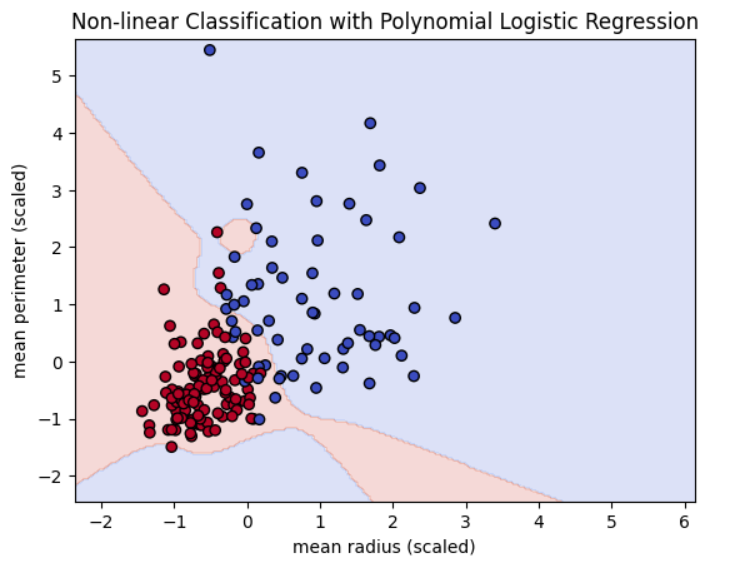
\includegraphics[scale=0.75]{img/203-4}

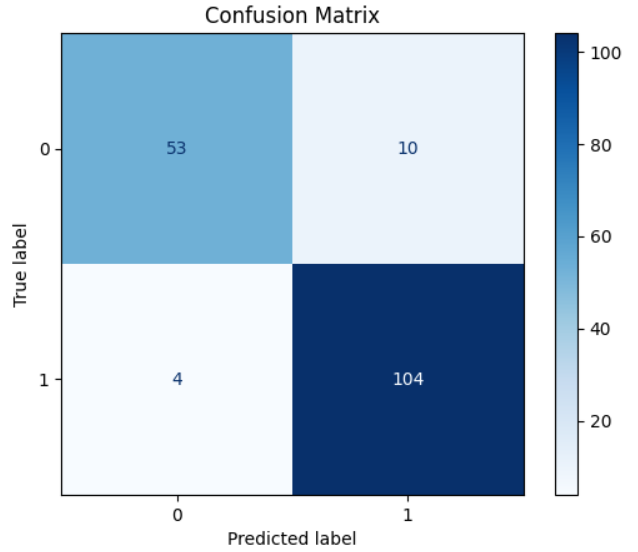
\includegraphics[scale=0.75]{img/203-5}



\section{Метод Опорних Векторів.}

Метод опорних векторів (Support Vector Machine) — це алгоритм класифікації, який шукає оптимальну гіперплощину, що розділяє дані двох класів із максимальним зазором (margin).

Нехай ми маємо навчальну вибірку:

$${(x_i, y_i)}_{i=1}^n, \quad x_i \in \mathbb{R}^d, \quad y_i \in \{-1, +1\}$$

Ми шукаємо гіперплощину, яка має вигляд:

$$w^T x + b = 0$$

де $w$ — вектор ваг (нормаль до гіперплощини), а $b$ — зсув (bias).


\textit{Умова коректної класифікації}: Для всіх навчальних точок повинно виконуватись:

$$y_i (w^T x_i + b) \ge 1$$

Це означає, що всі точки знаходяться по правильний бік гіперплощини, причому на відстані не менше 1 від неї.

*Відстань (margin)*: Відстань від точки до гіперплощини дорівнює:

$$
\frac{|w^T x + b|}{|w|}
$$

Ми хочемо максимізувати цей зазор між класами.
Для двох крайніх точок зазор дорівнює:

$$
\text{margin} = \frac{2}{|w|}
$$

Отже, щоб його максимізувати, потрібно мінімізувати $|w|^2$.


\textit{Оптимізаційна задача (лінійно роздільний випадок)}:

$$
\begin{aligned}
\min_{w, b} \quad & \frac{1}{2}|w|^2 \
\text{за умови:} \quad & y_i (w^T x_i + b) \ge 1, \quad i = 1, \dots, n
\end{aligned}
$$

Це опукла квадратична задача оптимізації. У реальних даних можливі помилки класифікації, тому вводять змінні послаблення $\xi_i \ge 0$:

$$
\begin{aligned}
\min_{w, b, \xi} \quad & \frac{1}{2}|w|^2 + C \sum_{i=1}^n \xi_i \
\text{за умови:} \quad & y_i (w^T x_i + b) \ge 1 - \xi_i, \quad i = 1, \dots, n
\end{aligned}
$$

де $C > 0$ — параметр, що задає компроміс між шириною зазору та кількістю помилок.


\textit{Ядровий трюк (kernel trick)}: Уявимо собі, що перед нами стоїть така задача: потрібно провести класифікацію температури на комфортну та некомфортну для людини. Якщо для людини комфортною температурою є 20 градусів за Цельсієм, то некомфортною є як -10 так і 40 градусів. Провести таку гіперплощину через ці дані, щоб всі точки з комфортною температурою були з однієї сторони, є неможливим. 

Для того, щоб провести гіперплощину в цьому випадку, ми можемо застосувати перетворення $y(x) = (x-20)^{2}$. Тоді всі некомфортні температури переходять у значення, більші за якесь $a$, тоді як всі комфортні температури відображаються у точки $x\leq a$. Це і є ядровий трюк.

Щоб працювати з нелінійно роздільними даними, SVM використовує перетворення простору:

$$\phi: \mathbb{R}^d \rightarrow \mathbb{R}^m$$

але замість явного обчислення $\phi(x)$ застосовується ядро $K(x_i, x_j) = \langle \phi(x_i), \phi(x_j) \rangle$.

Типові ядра, які використовуються для методу опорних векторів: лінійне ($K(x, x') = x^T x' $), поліноміальне ($K(x, x') = (x^T x' + 1)^d$)
та радіально-базисне (RBF, $K(x, x') = \exp(-\gamma |x - x'|^2) $ - це ядро використовується найчастіше).

Рішення у вигляді опорних векторів: у результаті оптимізації маємо:

$$f(x) = \text{sign}\left(\sum_{i=1}^n \alpha_i y_i K(x_i, x) + b\right)$$

де $\alpha_i$ — коефіцієнти лагранжа. Точки, для яких $\alpha_i > 0$, називаються опорними векторами — саме вони визначають гіперплощину.


\ding{43} Геометрична інтерпретація методу опорних векторів: SVM шукає межу, яка найбільше віддалена від найближчих точок обох класів. Тільки кілька опорних векторів визначають положення цієї межі.

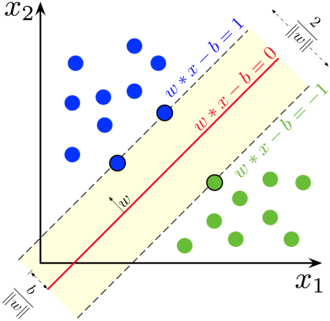
\includegraphics[scale=0.75]{img/ml-nonlinear-2}

Модуль для класифікації методом опорних векторів імпортується з пакету sklearn:

\begin{lstlisting}
from sklearn.svm import SVC
\end{lstlisting}

Тип ядра двказується через параметр \verb|kernel|:

\begin{lstlisting}
clf = SVC(kernel='rbf')
clf.fit(X_train_scaled, y_train)
\end{lstlisting}

Повністю код методу опорних векторів для задачі класифікації на датасеті пухлин молочної залози:

\begin{lstlisting}
import numpy as np
import matplotlib.pyplot as plt
from sklearn.datasets import load_breast_cancer
from sklearn.preprocessing import StandardScaler
from sklearn.svm import SVC
from sklearn.model_selection import train_test_split
from sklearn.metrics import ConfusionMatrixDisplay, accuracy_score

data = load_breast_cancer()
X = data.data[:, [3, 25]] 
y = data.target

X_train, X_test, y_train, y_test = train_test_split(X, y, test_size=0.3, random_state=42)

scaler = StandardScaler()
X_train_scaled = scaler.fit_transform(X_train)
X_test_scaled = scaler.transform(X_test)

clf = SVC(kernel='rbf')
clf.fit(X_train_scaled, y_train)

y_pred = clf.predict(X_test_scaled)
print("Accuracy:", accuracy_score(y_test, y_pred))

x_min, x_max = X_train_scaled[:, 0].min() - 1, X_train_scaled[:, 0].max() + 1
y_min, y_max = X_train_scaled[:, 1].min() - 1, X_train_scaled[:, 1].max() + 1
xx, yy = np.meshgrid(np.linspace(x_min, x_max, 200),
                     np.linspace(y_min, y_max, 200))

Z = clf.predict(np.c_[xx.ravel(), yy.ravel()])
Z = Z.reshape(xx.shape)

plt.contourf(xx, yy, Z, alpha=0.2, cmap='coolwarm')
plt.scatter(X_test_scaled[:, 0], X_test_scaled[:, 1], c=y_test, cmap='coolwarm', edgecolors='k')
plt.xlabel('mean radius (scaled)')
plt.ylabel('mean perimeter (scaled)')
plt.title('Non-linear Classification with SVM (RBF kernel)')
plt.show()

ConfusionMatrixDisplay.from_predictions(y_test, y_pred, cmap='Blues')
plt.title("Confusion Matrix")
plt.show()
\end{lstlisting}

Результат:

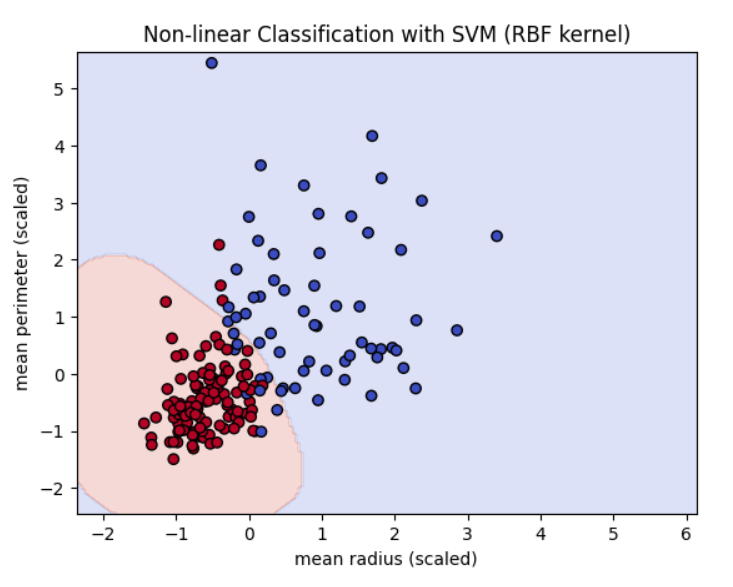
\includegraphics[scale=0.75]{img/203-6}

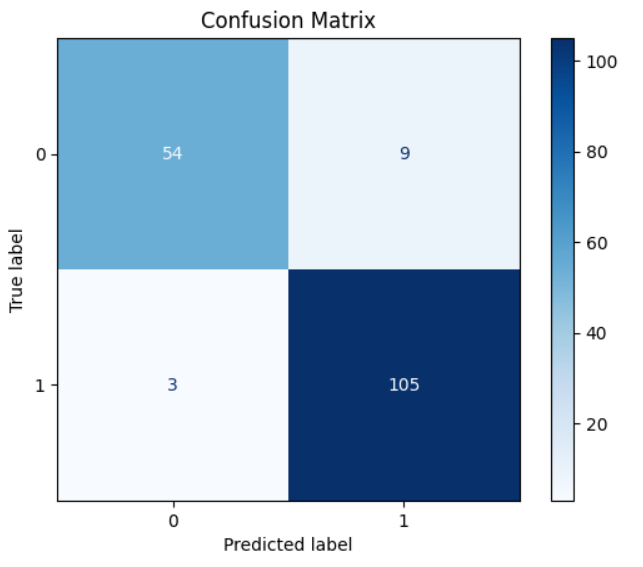
\includegraphics[scale=0.75]{img/203-7}


\section{Наївний баєсів класифікатор.}

Наївний баєсівський класифікатор (Naive Bayes classifier) — це ймовірнісний метод класифікації, який базується на теоремі Байєса.
Він оцінює, до якого класу належить об’єкт $ x $, обчислюючи ймовірність $P(C_k | x)$ для кожного класу $C_k$.

Теорема Байєса: основна формула

$$P(C_k | x) = \frac{P(x | C_k) , P(C_k)}{P(x)}$$

де $P(C_k | x)$ — апостеріорна ймовірність класу після спостереження ознак, $P(x | C_k)$ — правдоподібність (як імовірно отримати ознаки, якщо відомий клас), $P(C_k)$ — апріорна ймовірність класу, $P(x)$ — нормувальний коефіцієнт (спільна ймовірність ознак).

при цьому методі машинного навчання, ми робимо так зване \textit{"наївне" припущення незалежності}: методологічних вважає, що всі ознаки $x_1, x_2, \dots, x_n$ незалежні одна від одної, якщо відомо, до якого класу належить об’єкт.

$$P(x | C_k) = \prod_{j=1}^n P(x_j | C_k)$$

Це "наївне" припущення значно спрощує обчислення, навіть якщо насправді ознаки частково залежать.

Формула класифікації: Підставимо у формулу Байєса:

$$P(C_k | x) \propto P(C_k) \prod_{j=1}^n P(x_j | C_k)$$

Оскільки $ P(x) $ однакова для всіх класів, її можна не враховувати при порівнянні.

Отже, ми вибираємо клас з максимальною апостеріорною ймовірністю:

$$\hat{C} = \arg\max_{C_k} ; P(C_k) \prod_{j=1}^n P(x_j | C_k)$$

Наведемо приклад використання наївного баєсівого класифікатора для задачі класифікації пухлин:

\begin{lstlisting}
import numpy as np
import matplotlib.pyplot as plt
from sklearn.datasets import load_breast_cancer
from sklearn.preprocessing import StandardScaler
from sklearn.naive_bayes import GaussianNB
from sklearn.model_selection import train_test_split
from sklearn.metrics import ConfusionMatrixDisplay, accuracy_score

data = load_breast_cancer()
X = data.data[:, [3, 25]]  
y = data.target

X_train, X_test, y_train, y_test = train_test_split(
    X, y, test_size=0.3, random_state=42
)

scaler = StandardScaler()
X_train_scaled = scaler.fit_transform(X_train)
X_test_scaled = scaler.transform(X_test)

clf = GaussianNB()
clf.fit(X_train_scaled, y_train)

y_pred = clf.predict(X_test_scaled)
print("Accuracy:", accuracy_score(y_test, y_pred))

x_min, x_max = X_train_scaled[:, 0].min() - 1, X_train_scaled[:, 0].max() + 1
y_min, y_max = X_train_scaled[:, 1].min() - 1, X_train_scaled[:, 1].max() + 1
xx, yy = np.meshgrid(
    np.linspace(x_min, x_max, 200),
    np.linspace(y_min, y_max, 200)
)

Z = clf.predict(np.c_[xx.ravel(), yy.ravel()])
Z = Z.reshape(xx.shape)

plt.contourf(xx, yy, Z, alpha=0.2, cmap='coolwarm')
plt.scatter(X_test_scaled[:, 0], X_test_scaled[:, 1], c=y_test, cmap='coolwarm', edgecolors='k')
plt.xlabel('mean radius (scaled)')
plt.ylabel('mean perimeter (scaled)')
plt.title('Classification with Gaussian Naive Bayes')
plt.show()

ConfusionMatrixDisplay.from_predictions(y_test, y_pred, cmap='Blues')
plt.title("Confusion Matrix")
plt.show()
\end{lstlisting}

Результат:

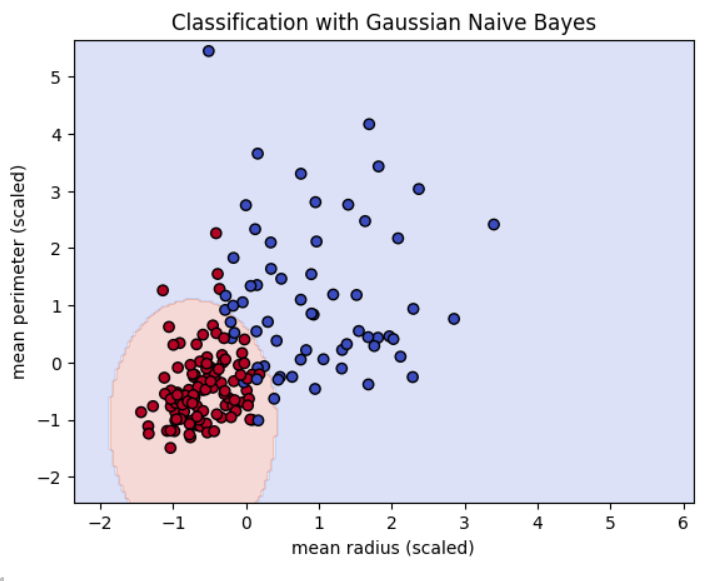
\includegraphics[scale=0.75]{img/203-8}

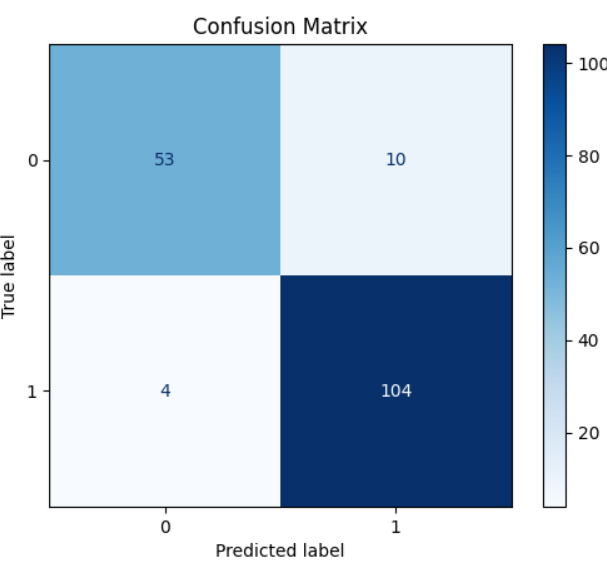
\includegraphics[scale=0.75]{img/203-9}



\section{Дерева прийняття рішень.}

Алгоритм дерева прийняття рішень (Decision trees) використовується для класифікації або регресії.
Його ідея — розділяти простір ознак на підмножини так, щоб отримати групи об’єктів, максимально однорідні за цільовою змінною.

Дерево прийняття рішень — це ієрархічна структура, де вузол (node) містить умову розділення (наприклад, $x_{i} < t$), гілки (branches) це варіанти переходу (так/ні), а листки (leaves) — фінальні рішення (клас або числове значення)

Нехай ми маємо навчальну вибірку:

$${(x_i, y_i)}_{i=1}^n, \quad x_i \in \mathbb{R}^d, ; y_i \in {1, 2, \dots, K}$$

Наша мета — знайти функцію $ f(x) $, яка розбиває простір ознак на області $ R_m $, і кожній області відповідає передбачення класу:

$$f(x) = \sum_{m=1}^{M} c_m \cdot I(x \in R_m)$$

де $ R_m $ — регіон (листок дерева), $c_m $ — значення або клас, який передбачається для цього регіону,  $ I(\cdot) $ — індикаторна функція (1, якщо умова виконується).

На кожному кроці вибирається ознака $ x_j $ та поріг $ t $, які найкраще поділяють дані на дві частини:

$$R_1(j, t) = {x \mid x_j \le t}, \quad R_2(j, t) = {x \mid x_j > t}$$

Ми вибираємо такі $j, t$, що мінімізують певну функцію втрат $L$.

Тут можна навести приклад із класифікацією пацієнтів за ризиком серцевих захворювань. Нехай перед нами стоїть задача класифікувати пацієнтів таким чином. Тут логічно будувати дерево, в якому на вузлах пацієнти будуть розділятися за віком (вік, більший за певне число - підвищений ризик), вагою (вага, більша за певне число - також ризик захворювань), та схильністю до куріння. Питання лише в підборі конкретних чисел (гранична вага та вік) таким чином, щоб мінімізувати ентропію (пацієнти, що будуть неправильно класифіковані). 

Як бачимо, дерево прийняття рішень є цілком інтуїтивно зрозумілим алгоритмом, а значною перевагою цієї моделі є її інтерпретованість.

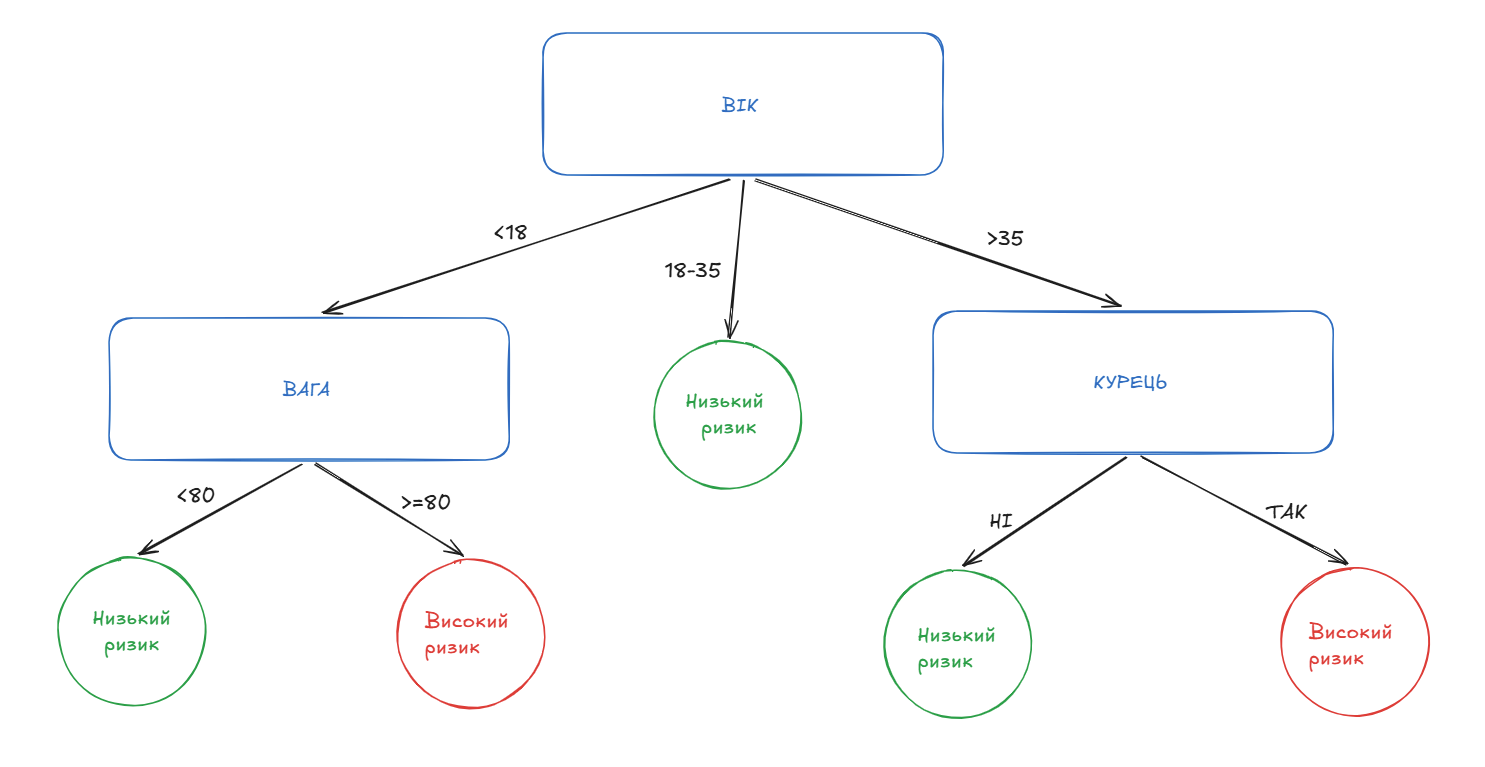
\includegraphics[scale=0.5]{img/203-12}

Приклад з використанням sklearn:

\begin{lstlisting}
import numpy as np
import matplotlib.pyplot as plt
from sklearn.datasets import load_breast_cancer
from sklearn.tree import DecisionTreeClassifier, plot_tree
from sklearn.model_selection import train_test_split

data = load_breast_cancer()

X = data.data[:, [3, 25]]
y = data.target

X_train, X_test, y_train, y_test = train_test_split(X, y, test_size=0.3, random_state=42)

clf = DecisionTreeClassifier(max_depth=5, criterion='gini', random_state=42)
clf.fit(X_train, y_train)

print("Accuracy on test set:", clf.score(X_test, y_test))

x_min, x_max = X[:, 0].min() - 0.01, X[:, 0].max() + 0.01
y_min, y_max = X[:, 1].min() - 0.01, X[:, 1].max() + 0.01
xx, yy = np.meshgrid(np.linspace(x_min, x_max, 300),
                     np.linspace(y_min, y_max, 300))

Z = clf.predict(np.c_[xx.ravel(), yy.ravel()])
Z = Z.reshape(xx.shape)

plt.figure(figsize=(10, 6))
plt.contourf(xx, yy, Z, alpha=0.3, cmap=plt.cm.RdYlBu)
scatter = plt.scatter(X[:, 0], X[:, 1], c=y, cmap=plt.cm.RdYlBu, edgecolor='k', s=50)

plt.xlabel(data.feature_names[3])
plt.ylabel(data.feature_names[25])
plt.title("Decision Tree Classifier (Depth=3)")
# plt.legend(handles=scatter.legend_elements()[0], labels=data.target_names)
plt.show()

plt.figure(figsize=(14, 8))
plot_tree(clf, feature_names=[data.feature_names[3], data.feature_names[25]],
          class_names=data.target_names, filled=True, rounded=True)
plt.title("Decision Tree Structure (2 features)")
plt.show()
\end{lstlisting}

Результат:

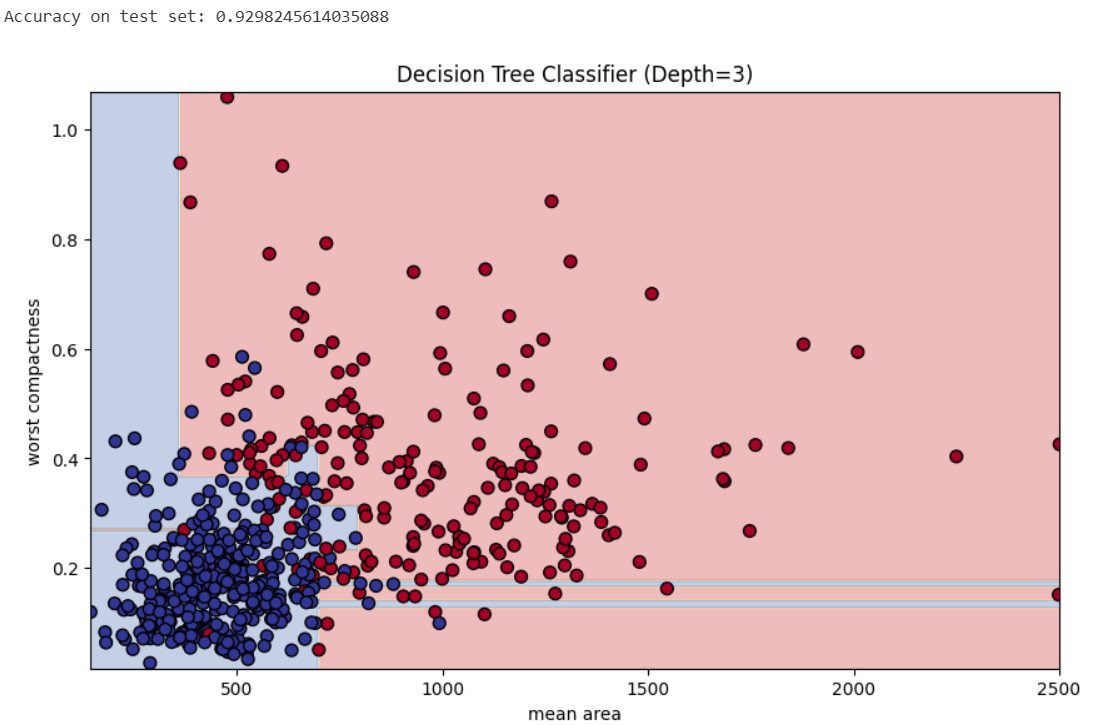
\includegraphics[scale=0.75]{img/203-10}

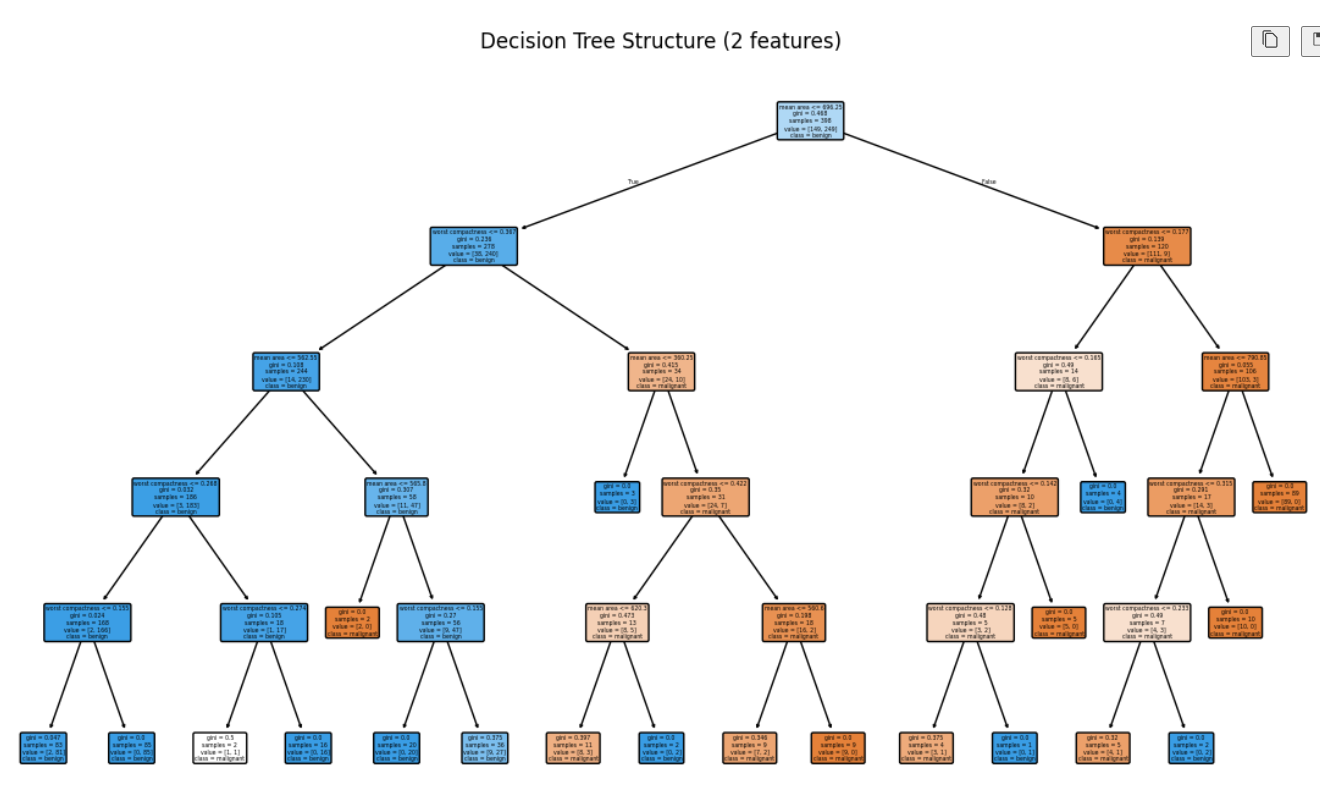
\includegraphics[scale=0.5]{img/203-11}


\ding{46} \textbf{Питання для самоконтролю.}

\begin{enumerate}
\item Що таке нелінійна модель машинного навчання?
\item Чим нелінійні моделі відрізняються від лінійних?
\item Які переваги мають нелінійні алгоритми?
\item Які недоліки можуть виникати під час використання нелінійних моделей?
\item У яких випадках лінійних моделей недостатньо?
\item Що таке складність моделі?
\item Як складність моделі впливає на її здатність до узагальнення?
\item Що таке поліноміальна регресія?
\item Чому поліноміальна регресія вважається нелінійною моделлю?
\item Як формується поліноміальна ознака другого степеня?
\item Як виглядає рівняння поліноміальної регресії другого порядку?
\item Для чого використовуються поліноміальні ознаки?
\item Як вибір степеня полінома впливає на модель?
\item Які переваги має поліноміальна регресія?
\item Які недоліки має поліноміальна регресія?
\item Що відбувається при надто великому степені полінома?
\item Як поліноміальна регресія може призвести до перенавчання?
\item Що таке узагальнююча здатність моделі?
\item Що таке перенавчання (Overfitting)?
\item Які ознаки свідчать про перенавчання моделі?
\item Що таке недонавчання (Underfitting)?
\item Чим перенавчання відрізняється від недонавчання?
\item Які причини виникнення перенавчання?
\item Як кількість ознак впливає на ризик перенавчання?
\item Які методи використовують для боротьби з перенавчанням?
\item Чому важливо оцінювати модель на даних, які не використовувались під час навчання?
\item Що таке перехресна валідація (Cross-Validation)?
\item Для чого використовується k-кратна перехресна валідація?
\item Як працює метод k-fold cross-validation?
\item Що означає параметр k у k-fold validation?
\item Які переваги має перехресна валідація порівняно зі звичайним поділом даних?
\item Як обчислюється підсумкова якість моделі при k-fold validation?
\item Як вибір значення k впливає на результати оцінювання?
\item Чому k-кратна перехресна валідація допомагає виявляти перенавчання?
\item Що таке поліноміальна класифікація?
\item Як поліноміальні ознаки дозволяють будувати нелінійні межі класифікації?
\item Чим поліноміальна класифікація відрізняється від лінійної?
\item Які переваги має використання поліноміальних ознак у класифікації?
\item Що таке метод опорних векторів (Support Vector Machine)?
\item Яка основна ідея алгоритму SVM?
\item Що таке гіперплощина класифікації в SVM?
\item Що таке опорні вектори?
\item Що називають відступом (margin) між класами?
\item Чому SVM прагне максимізувати margin?
\item Для чого використовується ядро (kernel) в SVM?
\item Які типи ядер найчастіше використовуються в SVM?
\item Як ядровий трюк (Kernel Trick) дозволяє будувати нелінійні класифікатори?
\item Що таке наївний баєсівський класифікатор?
\item На якій математичній теоремі базується цей алгоритм?
\item У чому полягає припущення про незалежність ознак?
\item Чому класифікатор називають «наївним»?
\item Які переваги має наївний баєсівський класифікатор?
\item Які недоліки має наївний баєсівський підхід?
\item У яких задачах особливо часто застосовують Naive Bayes?
\item Чому цей алгоритм популярний у задачах обробки тексту?
\item Що таке дерево прийняття рішень?
\item З яких основних елементів складається дерево рішень?
\item Що таке кореневий вузол дерева?
\item Що таке внутрішній вузол дерева?
\item Що таке лист дерева?
\item Як дерево приймає рішення щодо класифікації об'єкта?
\item Що таке критерій розбиття вузла?
\item Для чого використовується ентропія під час побудови дерева?
\item Що таке Information Gain?
\item Як індекс Джині (Gini Index) використовується при побудові дерева?
\item Які переваги мають дерева прийняття рішень?
\item Які недоліки мають дерева прийняття рішень?
\item Чому дерева схильні до перенавчання?
\end{enumerate}


